\subsection*{Problema 10}

\textbf{Enunciado:} Calcular la integral:
\begin{align*}
\int \dfrac{x^3 + x^2 + x + 3}{x^4 + 4x^2 + 3} \, dx
\end{align*}

\textbf{Solución:} El denominador se puede factorizar como indica la sugerencia:
\begin{align*}
x^4 + 4x^2 + 3 = (x^2 + 1)(x^2 + 3)
\end{align*}

Planteamos la descomposición en fracciones parciales:
\begin{align*}
\dfrac{x^3 + x^2 + x + 3}{(x^2 + 1)(x^2 + 3)} &= \dfrac{Ax + B}{x^2 + 1} \\
&+ \dfrac{Cx + D}{x^2 + 3}
\end{align*}

Multiplicando por el denominador común, obtenemos:
\begin{align*}
x^3 + &x^2 + x + 3 = (Ax + B)(x^2 + 3) \\
&+ (Cx + D)(x^2 + 1)
\end{align*}

Expandiendo y agrupando términos según las potencias de $x$:
\begin{align*}
x^3 + x^2 + x + 3 &= (A + C)x^3 \\
&+ (B + D)x^2 \\
&+ (3A + C)x + (3B + D)
\end{align*}

Igualando los coeficientes de ambos lados de la ecuación, formamos el sistema:
\begin{align*}
A + C &= 1 \\
B + D &= 1 \\
3A + C &= 1 \\
3B + D &= 3
\end{align*}

Resolviendo el sistema para las variables:
\begin{align*}
\text{De } 3A + C &= 1 \text{ y } A + C = 1: \\
2A &= 0 \implies A = 0, \ C = 1 \\
\text{De } 3B + D &= 3 \text{ y } B + D = 1: \\
2B &= 2 \implies B = 1, \ D = 0
\end{align*}

Sustituyendo los valores hallados en las fracciones parciales:
\begin{align*}
\int \dfrac{1}{x^2 + 1} \, dx + \int \dfrac{x}{x^2 + 3} \, dx
\end{align*}

Calculando cada integral por separado, la primera es inmediata y la segunda requiere una sustitución $u = x^2 + 3$:
\begin{align*}
\int \dfrac{1}{x^2 + 1} \, dx &= \arctan(x) \\
\int \dfrac{x}{x^2 + 3} \, dx &= \dfrac{1}{2} \ln|x^2 + 3|
\end{align*}

Combinando los resultados y añadiendo la constante de integración $C$:
\begin{align*}
\int \dfrac{x^3 + x^2 + x + 3}{x^4 + 4x^2 + 3} \, dx = \\
\arctan(x) + \dfrac{1}{2} \ln(x^2 + 3) + C
\end{align*}

\begin{figure}[H]
	\centering
	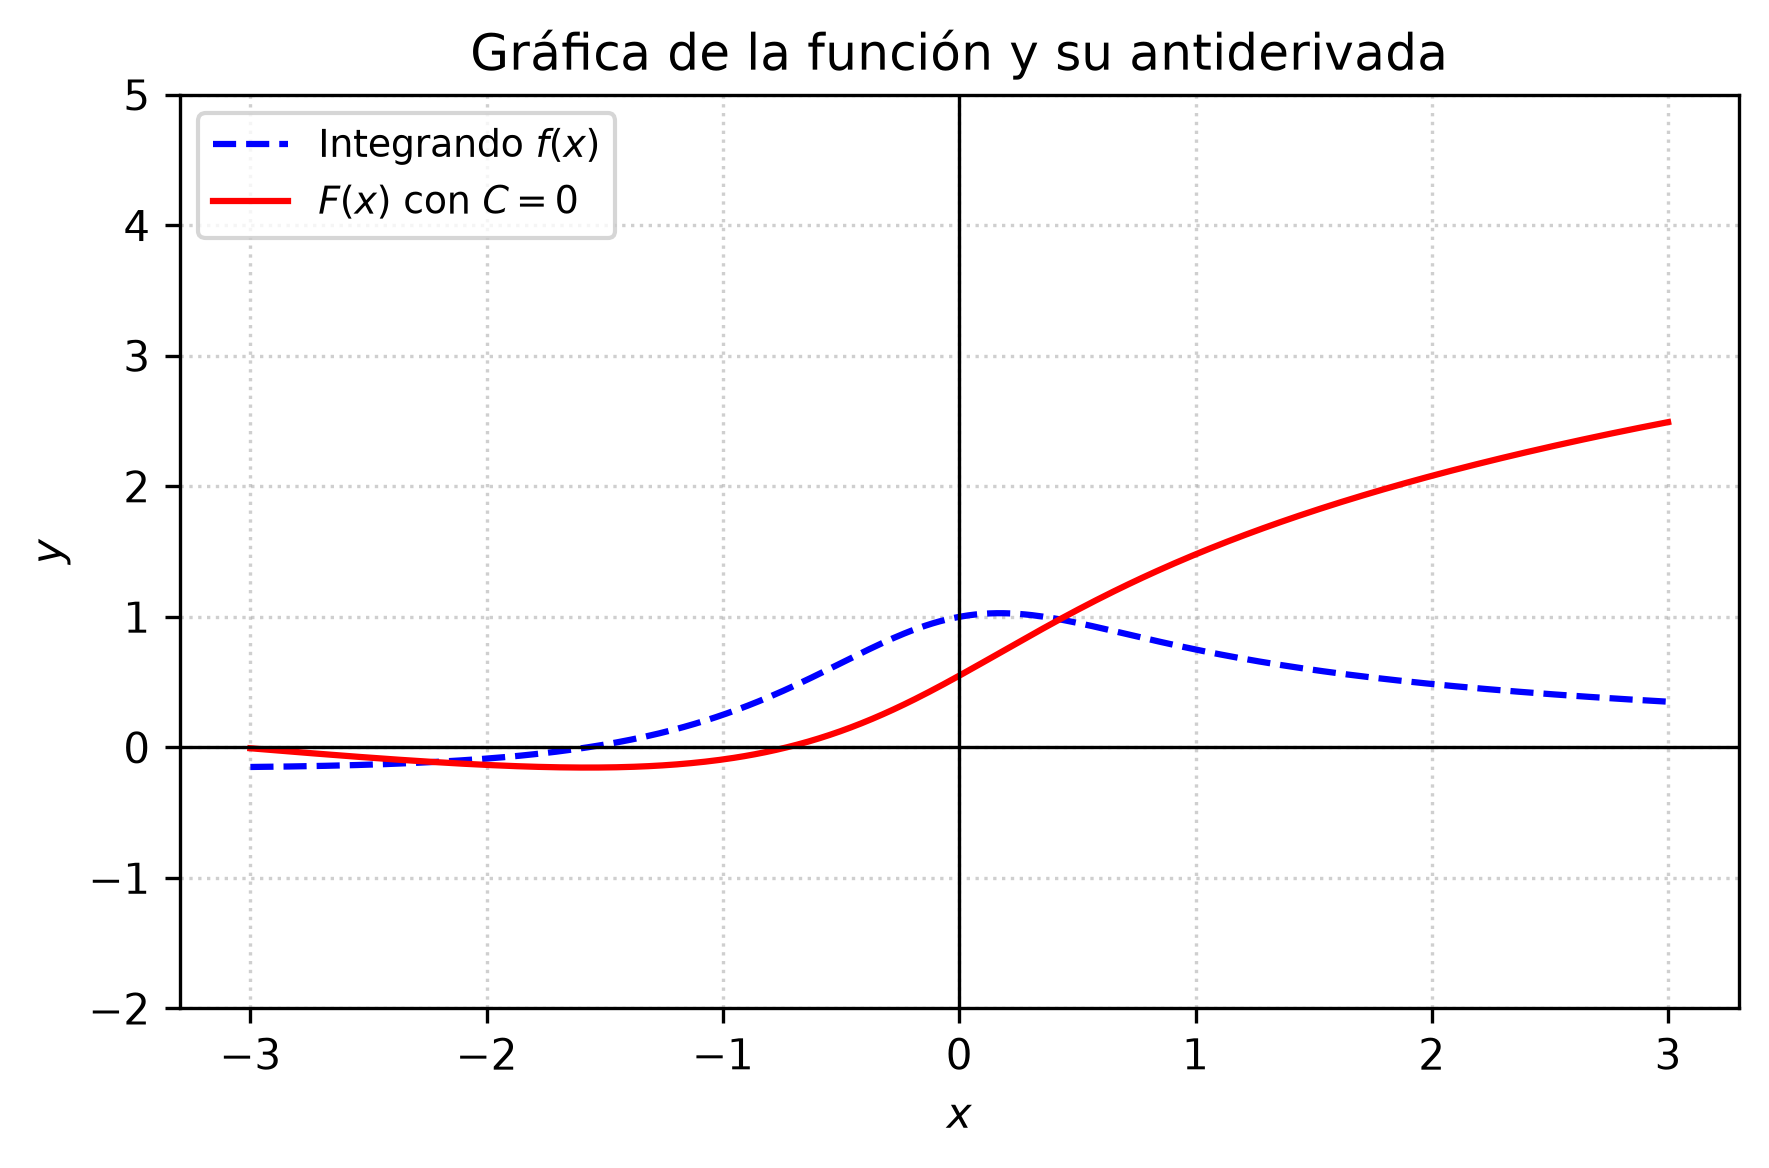
\includegraphics[width=\columnwidth]{semana_03/graficas/SEM03_P10_grafica.png}
	\caption{Representación gráfica de $f(x)$ y su antiderivada $F(x)$ evaluada para la constante de integración $C = 0$ (Problema 10).}
	\label{fig:problema10}
\end{figure}
